\begin{figure}[htp] \centering
        \begin{subfigure}[b]{0.5\columnwidth}
        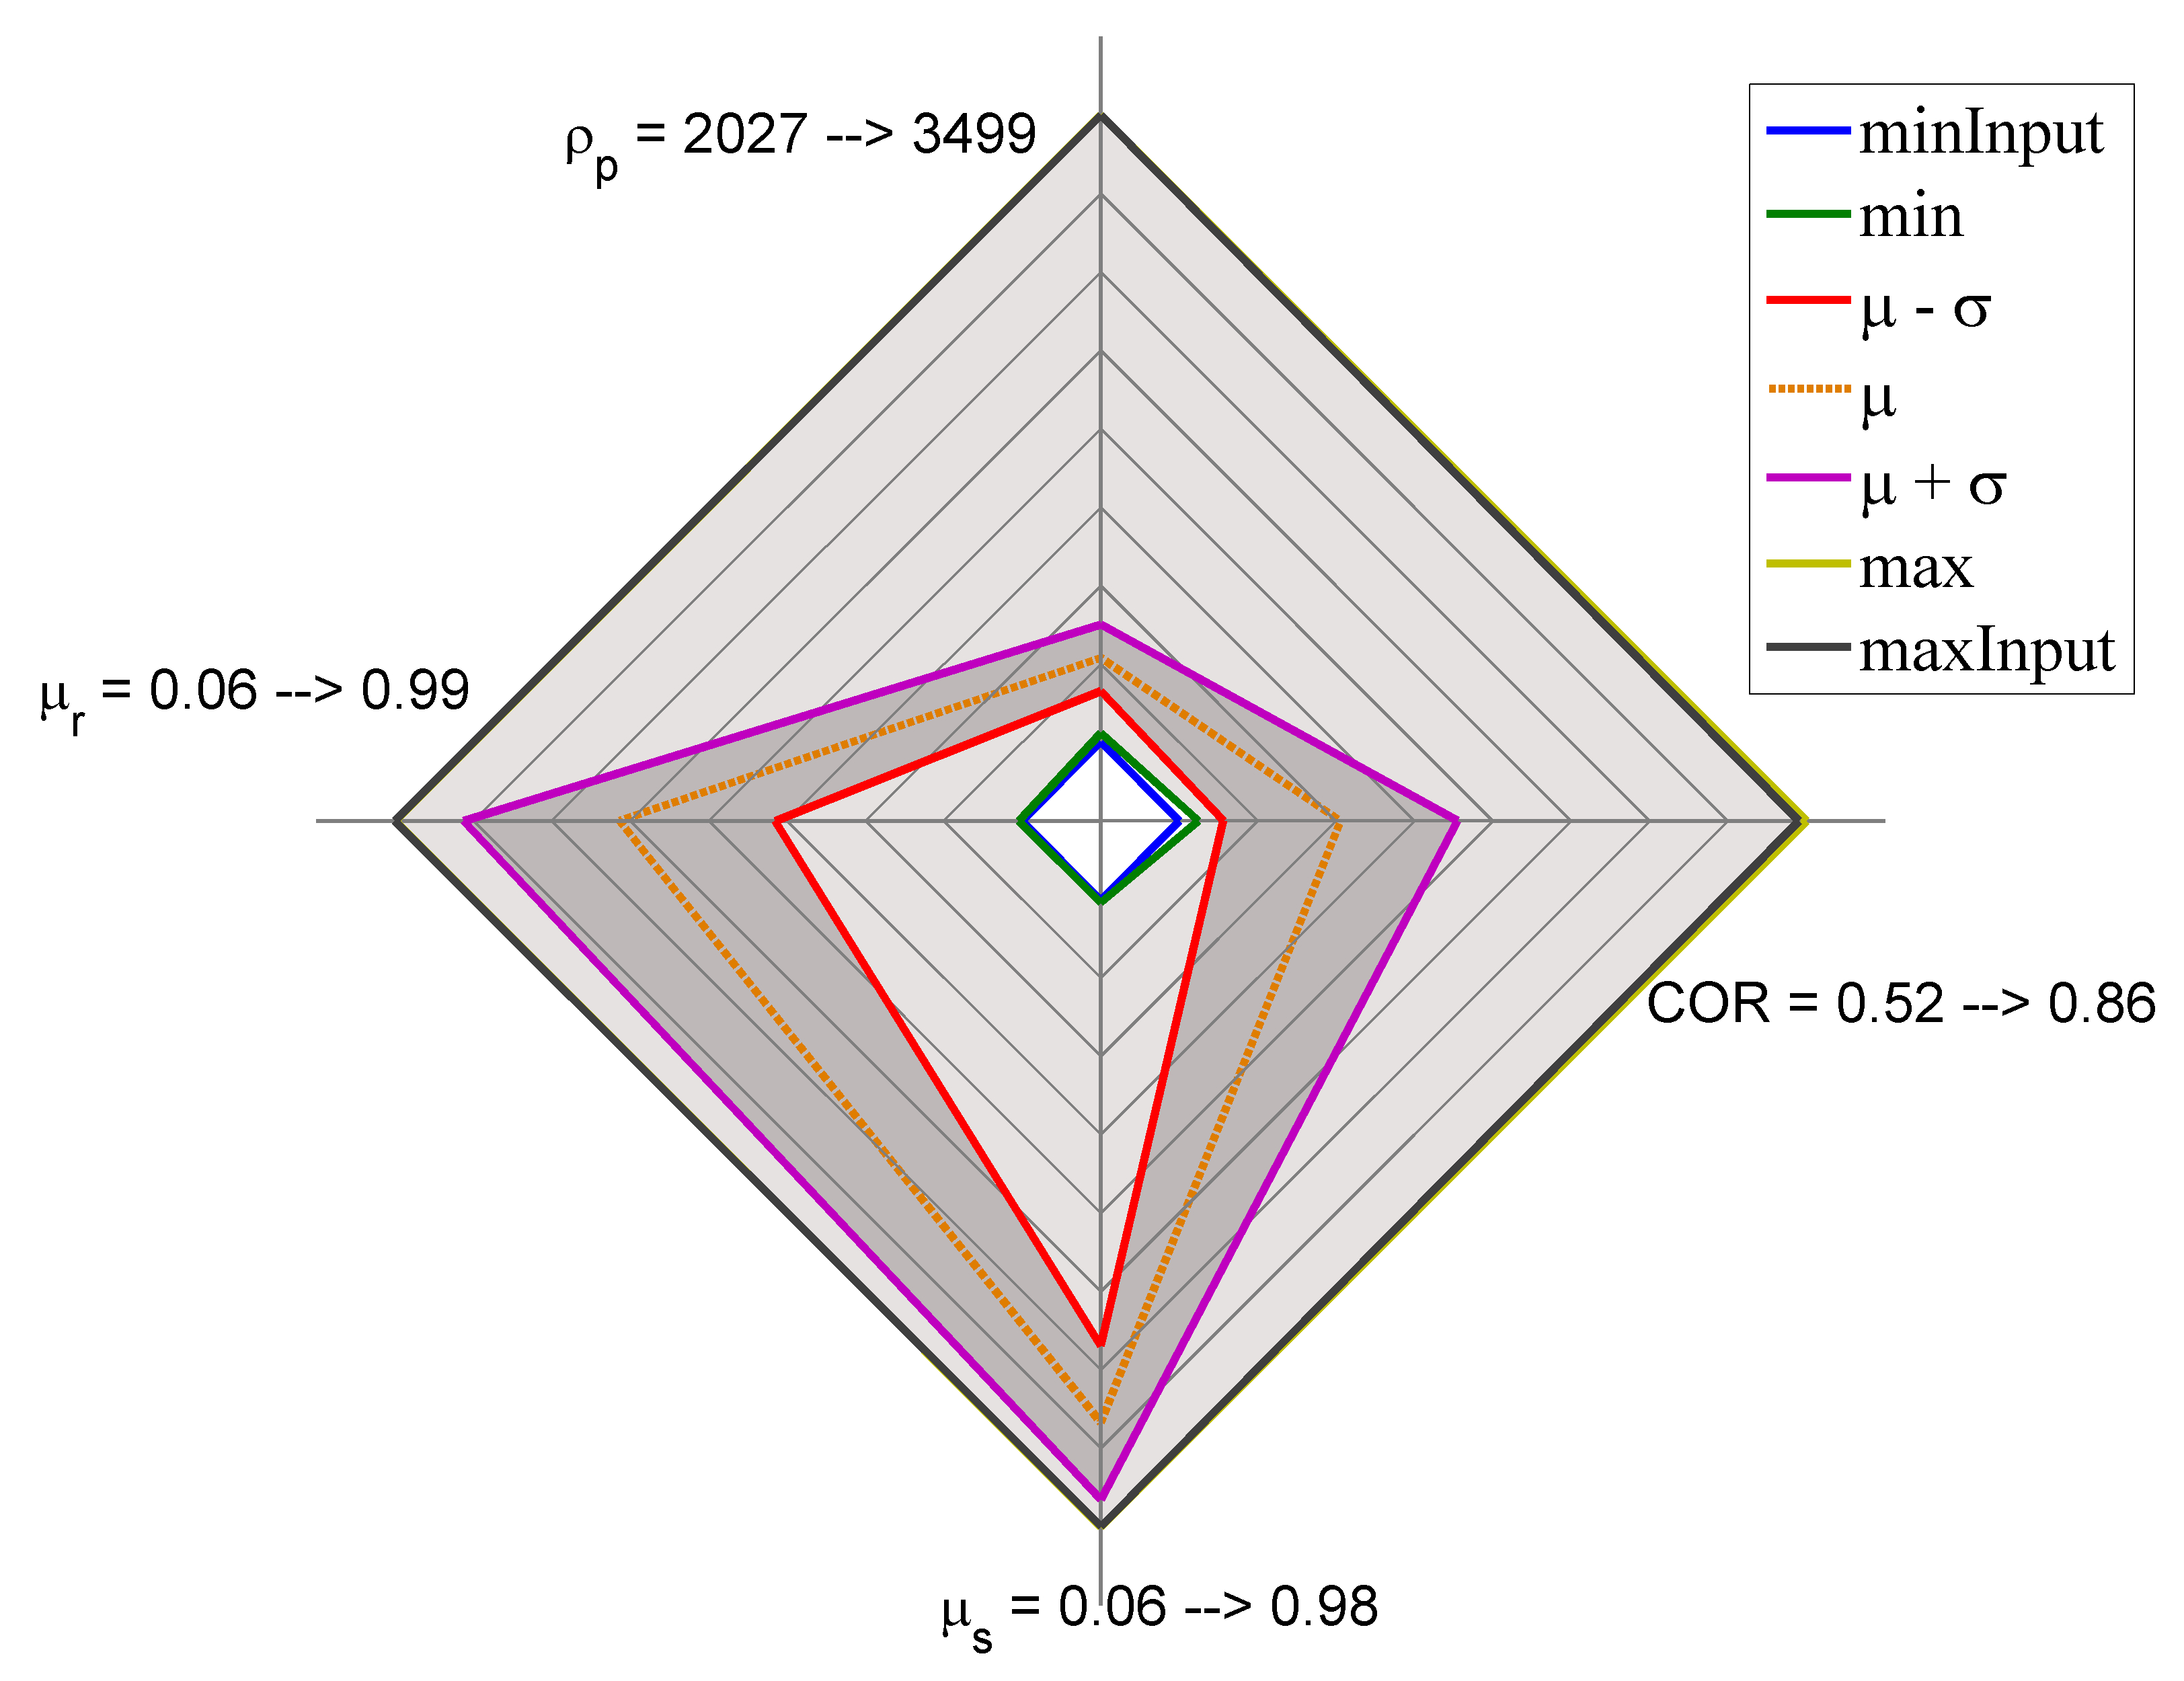
\includegraphics[width=\textwidth]{26radarpirker08schulze10070}
        \caption{Parameter space plot, $SSC$, $\sigma_n=10070 ~[Pa]$, $P=0.8$}
        \label{fig:26radarpirker08schulze10070} 
    \end{subfigure}\\
     \begin{subfigure}[b]{0.5\columnwidth}
        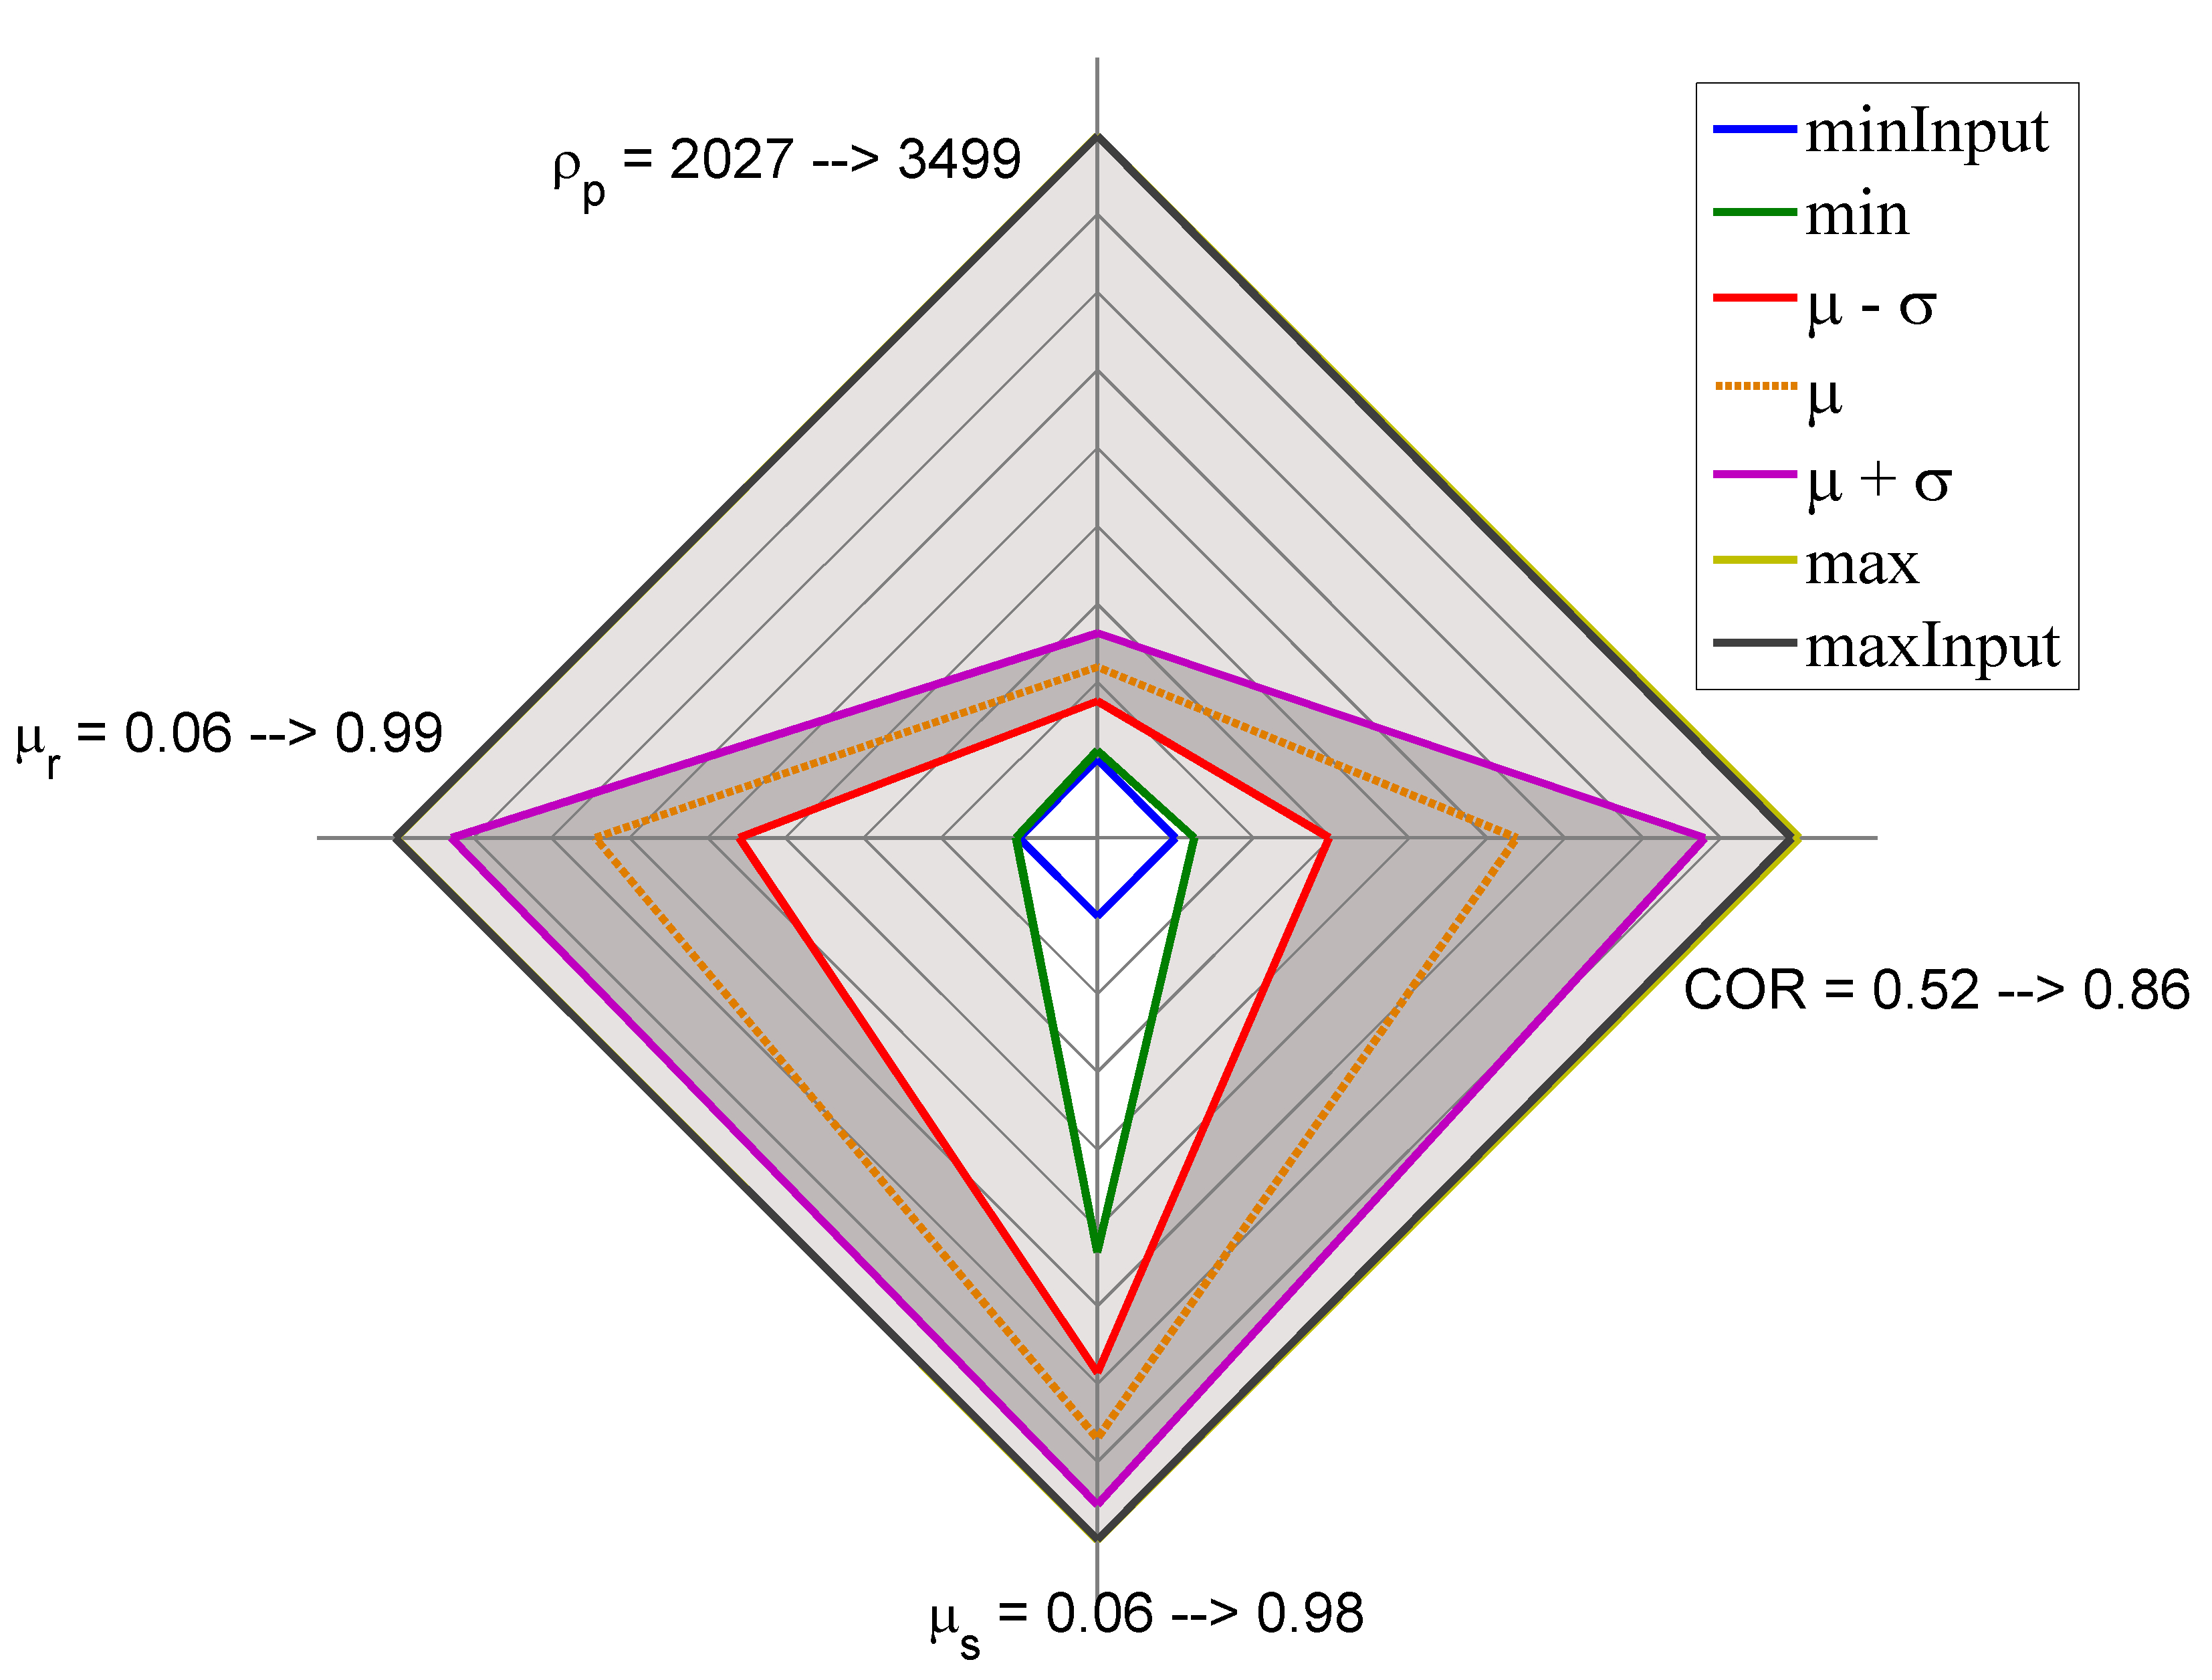
\includegraphics[width=\textwidth]{24radarpirker1schulze10070}
        \caption{Parameter space plot, $SSC$, $\sigma_n=10070 ~[Pa]$, $P=1.0$}
        \label{fig:24radarpirker1schulze10070}
    \end{subfigure} \\
        \begin{subfigure}[b]{0.5\columnwidth}
        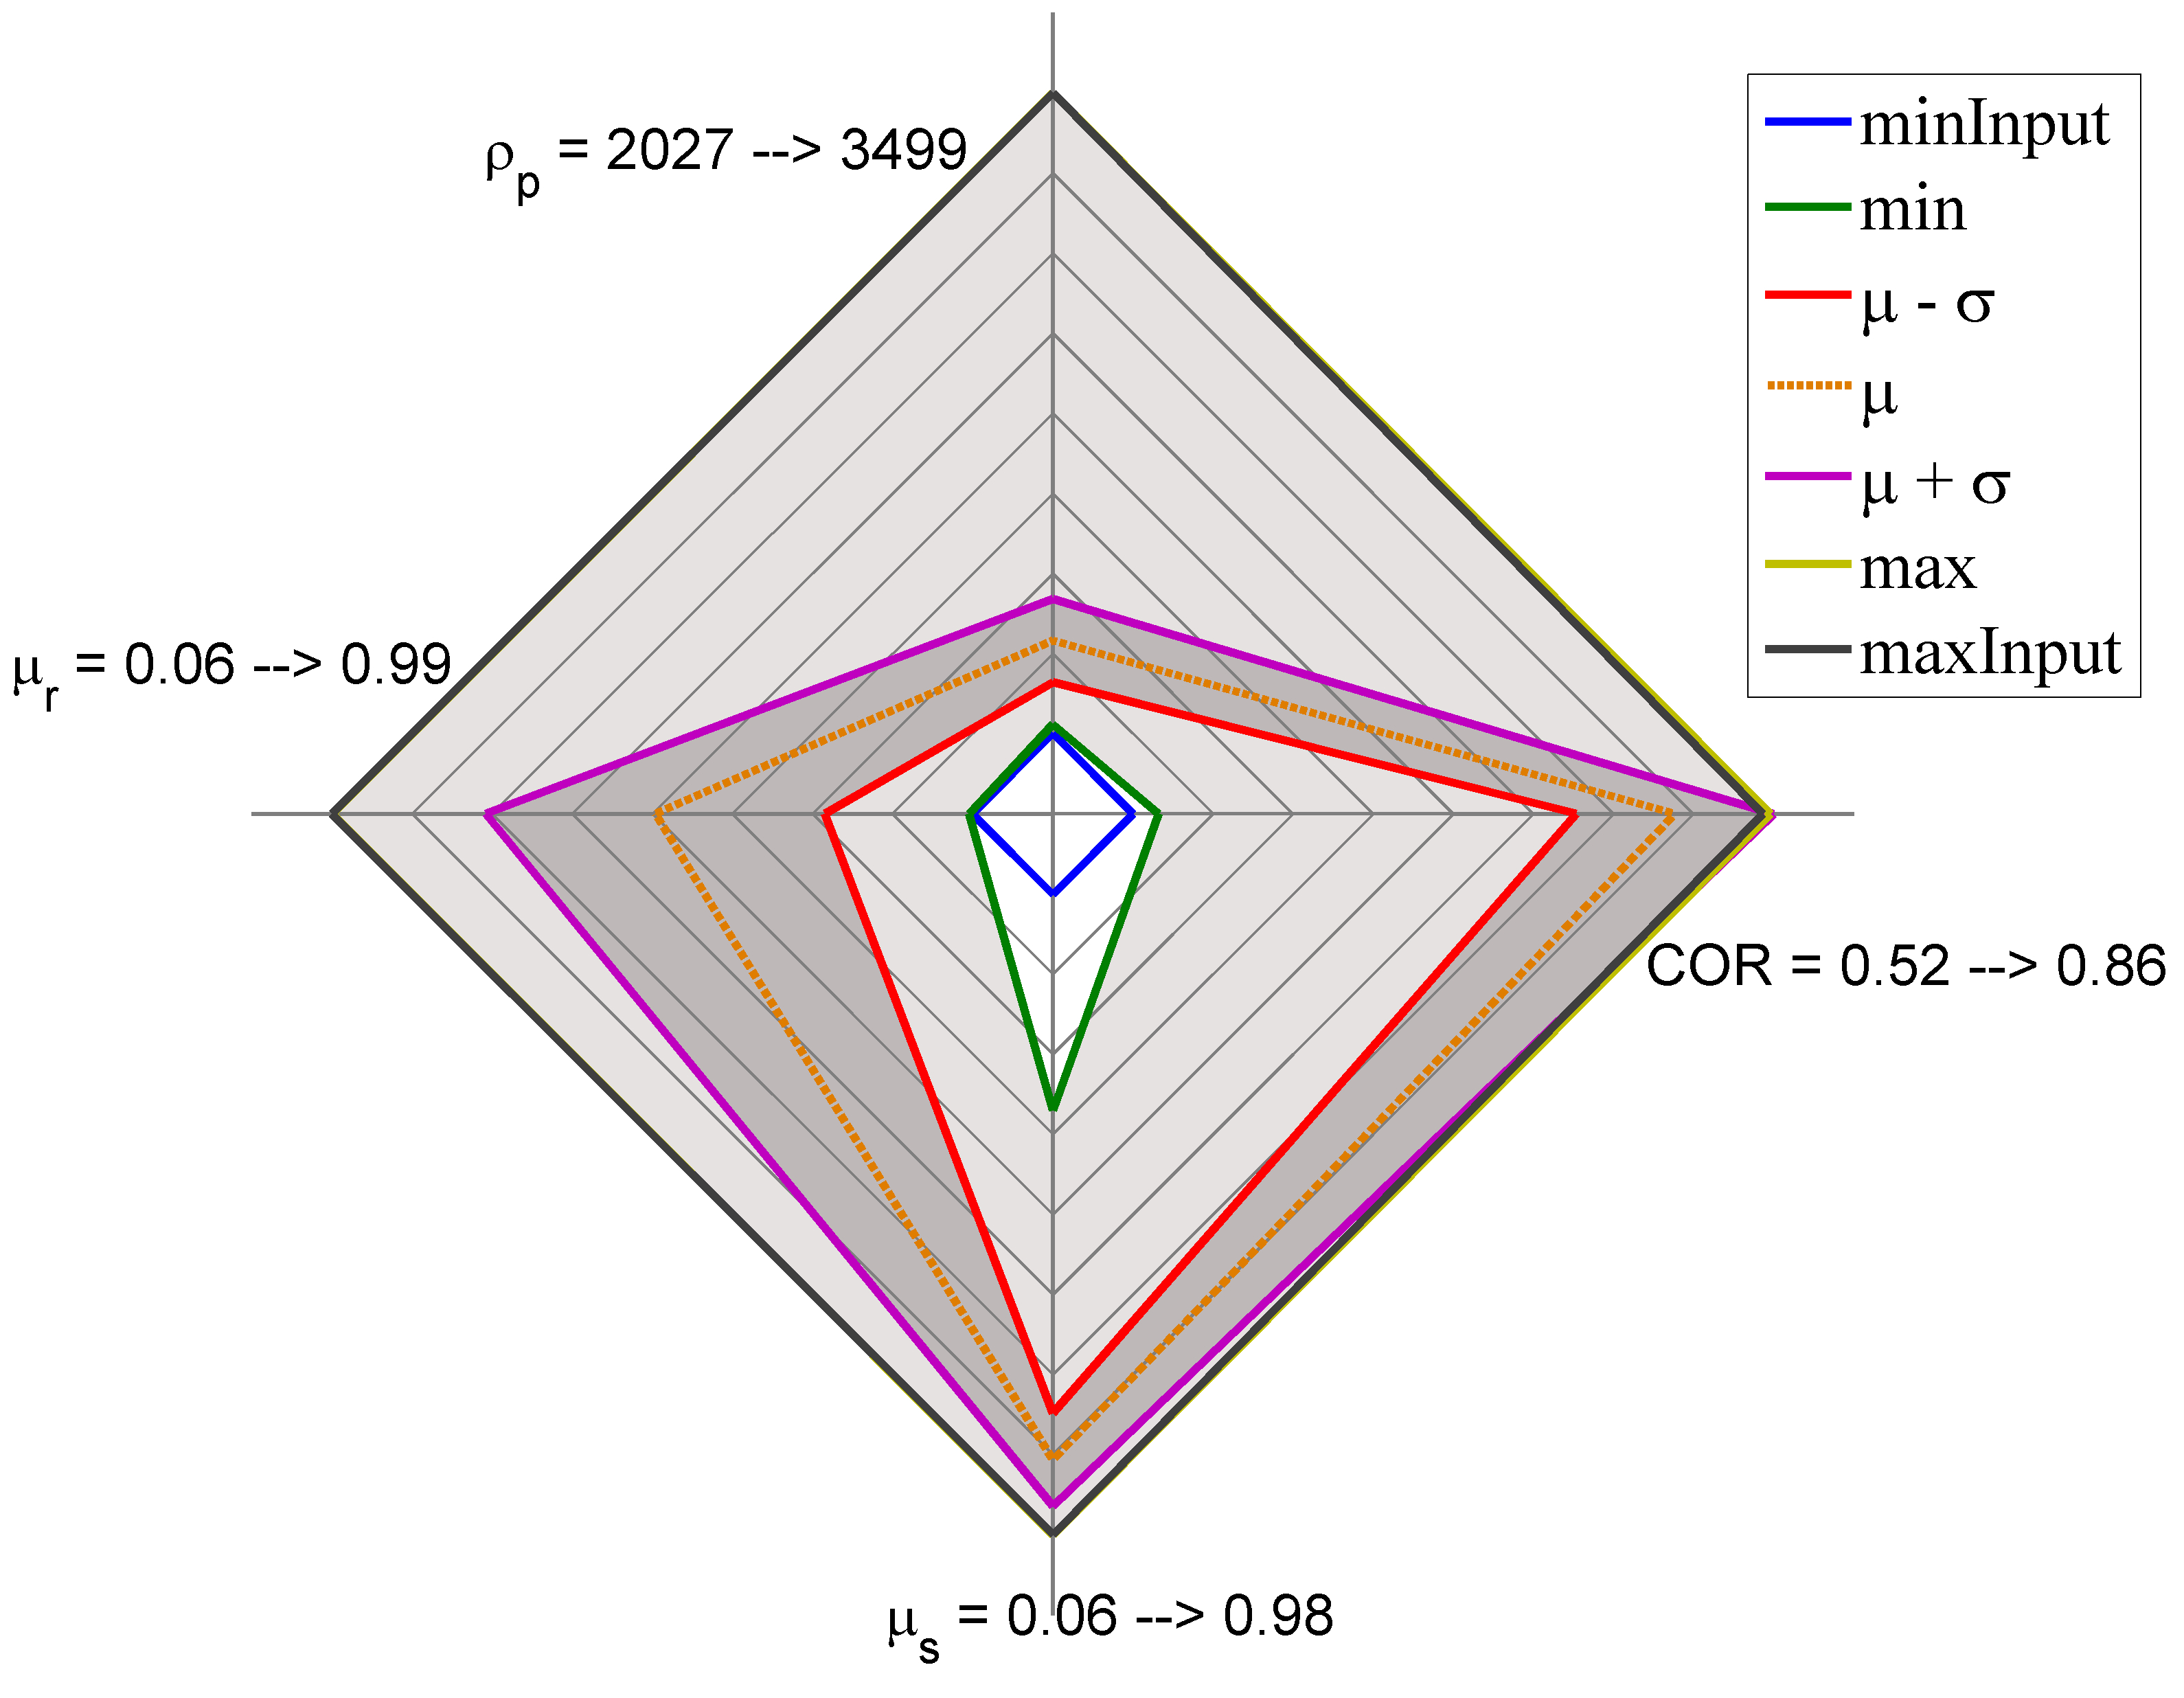
\includegraphics[width=\textwidth]{28radarpirker12schulze10070}
        \caption{Parameter space plot, $SSC$, $\sigma_n=10070 ~[Pa]$, $P=1.2$}
        \label{fig:28radarpirker12schulze10070} 
    \end{subfigure}
    \caption[Parameter space plot of valid simulations parameters for three different
    bulk behaviours measured by SCT]{Parameter space plot of valid simulations
    parameters for three different bulk behaviours measured by shear cell tester ($SSC$).
    Each axis of the parameter space plot represents one simulation parameters.
    Furthermore, the shaded area represents valid parameters combinations.
    Dark shaded values stand for the confidence range.
    We represent the marked combinations for one load condition of the shear
    cell.
    Further explanation in the text.
   }
    \label{fig:29schulzeradarandcloud}
\end{figure}